\chapter{Backgrounds}
\label{chap:backgrounds}
	\textit{This chapter introduces the background knowledge of this thesis, including information about Web Application Firewalls, Machine Learning Models and Deep Neural Networks.}
\minitoc

\section{Web Application Firewall} 
\label{sec:waf}
	
\subsection{What is WAF ?}
\label{subsec:waf_def}
WAF\index{WAF} stands for \textbf{Web Application Firewall}. This firewall solution commonly monitors data packets and filters them for the presence of malware or viruses. It performs the data monitoring/filtering for to and from data packets.  

The WAF tool can be distributed using network-based, cloud-based, or host-based architectures. It needs a reverse proxy to make sure that one or more web apps are in front of it while facing forward. 

It can be utilized either alone or in conjunction with other applications. WAF may function at a lower level or a higher level depending on the requirement\footnote{\label{wallarm} Wallarm. \textit{WAF Meaning}. \url{https://www.wallarm.com/what/waf-meaning}}.


\subsection{How does WAF work?}
\label{subsec:waf_work}
As previously stated, WAF is deployed at the application layer and serves as a two-way firewall. At work, WAF monitors HTTP or HTTPS traffic entering or exiting a specific web app. When WAF detects a malicious object in the traffic, it activates and destroys it. Figure 2.1 demonstrates how WAF works, legitimate users (top-left and bottom-left) are permitted access to the server with a WAF enabled, but attackers (middle-left) are prevented from doing so.
\begin{figure}[!h]
   
	\centering
	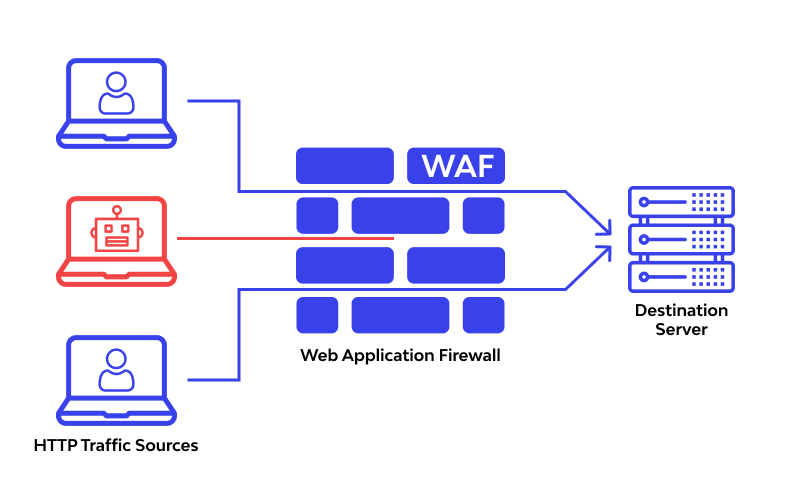
\includegraphics[width=\linewidth, height=7.5cm,keepaspectratio]{figures/wallarmwaf.png}
	\caption{How does WAF work.}\label{Fig:Data1}
  
\end{figure}
\\
WAF predefined what is malicious and what is not to make the process easier. WAF adheres to these guidelines throughout the process. WAF primarily analyzes the GET and POST portions of HTTP traffic. GET retrieves data from the server, whereas POST directs data to the server to change its original state\footnoteref{wallarm}.
% \footnote{Wallarm. \textit{WAF Meaning}. \url{https://www.wallarm.com/what/waf-meaning}}.
\subsection{WAF vs Firewall}
\label{subsec:versus}
In the modern era of sophisticated cyberattacks and digital innovation, it is essential for organizations to understand the threats they face and what their security measures protect them from. Understanding the value of and distinctions between WAF\index{WAF} security and network firewall security is vital for preventing online attacks and other types of network intrusions\footnote{Fortinet. \textit{WAF vs. Firewall: Web Application and Network Firewalls}. 
\url{https://www.fortinet.com/resources/cyberglossary/waf-vs-firewall}}.

A web application firewall (WAF) protects web applications by intercepting Hypertext Transfer Protocol (HTTP) traffic. This is distinct from a traditional firewall, which acts as a wall between external and internal network traffic.

A WAF stands between external users and web applications to track all HTTP traffic. It then identifies and stops harmful requests from entering users or apps on the web. As a result, WAFs protect key company online applications and servers from zero-day threats and other application-layer attacks. This becomes highly critical as firms invest in new digital efforts, which could expose new web apps and APIs to attacks.

A network firewall guards a secure local-area network against unwanted access to reduce the risk of assaults. Its goal is to distinguish a safe zone from a less secure zone and to control communication between the two. Without it, every device that has a public IP address is exposed to the outside network and potentially vulnerable to attack.

The layer of security that WAF and network-level firewalls operate on is the primary technological distinction between them. Attacks at OSI model Layer 7, or the application level, are protected by WAFs. This covers URL assaults, cookie manipulation, SQL injection, and attacks against JavaScript, ActiveX, and Ajax applications. They also target HTTP and HTTPS, the web application protocols that link web browsers and web servers. Network firewalls secure data transfer and network traffic at OSI model Layers 3 and 4. This covers assaults on the Domain Name System (DNS) and File Transfer Protocol (FTP), as well as Telnet, Secure Shell (SSH), and Simple Mail Transfer Protocol (SMTP). The following figure (Figure 2.2) displays the attacks which can be blocked by network firewall and WAF.
\begin{figure}[h!]
	\centering
	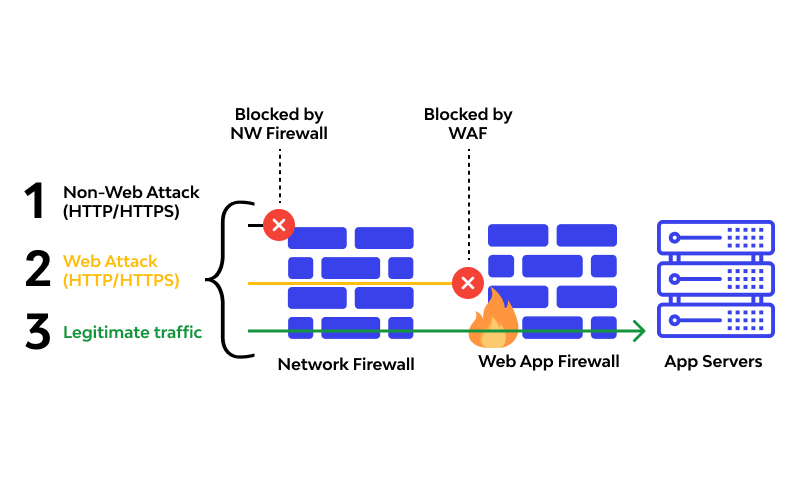
\includegraphics[width=\linewidth, height=8cm,keepaspectratio]{figures/waf3.png}
	\caption{Comparison between WAF and network firewall}
\end{figure}
\newpage

It's critical to pick a suitable network firewall or WAF\index{WAF} to protect against all of the risks that may be present. Businesses cannot be protected from web page attacks by a network firewall alone; WAF capabilities are the sole means of defense. Business organizations risk leaving their larger network vulnerable to attack due to web application vulnerabilities without an application firewall. A WAF cannot protect from attacks at the network layer, so it should supplement a network firewall rather than replace it. Network-based and web-based solutions operate at several layers and protect from multiple types of traffic. As a result, they perform best together rather than against one another. A network firewall usually protects a wider range of traffic types, but a WAF deals with a specific threat that a conventional strategy cannot handle. Having both options is therefore advisable, especially if a company's operating systems and the web interact frequently.
\subsection{False Positive}
\subsubsection{What is false positive ?}
An alert produced when there is no real danger is known as a false positive\index{False positive} (FP). In other words, it serves as a warning indicator but ultimately proves to be a false alarm. False positives may appear to be innocuous annoyances, but they can have harmful effects\footnote{Hannah Brice. \textit{The Dangers of False Positives in Cybersecurity and how to avoid them}. Oct 2022. 
\url{https://www.lupovis.io/the-dangers-of-false-positives-in-cybersecurity-and-how-to-avoid-them/}}.\\
For instance, when it discovers unusual behavior on a network, an intrusion detection system (IDS) may send out an alert. However, additional research reveals that the behavior is harmless—a false positive. For IT security teams who have to waste time looking into them, they are frequently the result of wrong settings or overly vigilant security software.
\newpage
Handling a large number of notifications is something that all WAF\index{WAF} specialists have experience with. They're probably also wasting a ton of time sorting out false positives from these warnings. Attacks are to be stopped, while valid traffic is to be allowed to pass through the WAF. False positive incidents clog the alerts feed and, worse yet, block legitimate traffic. A few false positive incidents happen because of flaws or poor application design. A WAF rule that is too general or doesn't fit the site's operation may trigger additional events\footnote{A. Lerner, N. Avital, S. Margel. 
\textit{Alert fatigue – introducing false positives in WAF}. Aug 2020.
\url{https://www.imperva.com/blog/avoid-alert-fatigue-how-to-automatically-get-rid-of-waf-false-positive/}}.
\subsubsection{The risks of false positive} 
Any expanding company will worry about scalability, and expanding development processes presents several difficulties. Small-scale development still frequently uses ad hoc toolkits and manual procedures, while the former can still produce too many false positives\index{False positive}.

The number of false positives can expand exponentially, and it is hard to handle them all manually, as upgrades, products, and workloads all continue to multiply.

There may be substantial financial repercussions as well. It can take too long to investigate reports that turn out to be false positives, which can result in delays and a possible loss of money and business possibilities.

Due to the overwhelming amount of false positives, staff members could grow accustomed to ignoring reports, increasing the likelihood that an actual vulnerability will go unnoticed and enter the production application, again with very costly results\footnote{Ritika Singh. \textit{The Risks Of False Positives With Web Application Firewalls}. Sep 2021. \url{https://www.indusface.com/blog/the-risks-of-false-positives-with-web-application-firewalls/}}.

\newpage
\section{Machine Learning Model} 
\label{sec:machine_model}
	
\subsection{Logistic Regression}
\label{subsec:logistic_regression}
\subsubsection{Logistic Regression Model}
Predictive output of Linear Regression:
\begin{align}
	f(x) = w^T x
\end{align}

\subsubsection{Sigmoid Function}
Sigmoid function:
\begin{align}
    f(s) = \frac{1}{1 + e^{-s}} \triangleq \sigma(s)
\end{align}

\subsubsection{Optimize loss function}
The Stochastic Gradient Descent (SGD) algorithm will be used here.

\begin{align}
    & \frac{\partial z}{z(1-z)} = \partial s \\ 
	\Leftrightarrow & (\frac{1}{z} + \frac{1}{1 - z})\partial z = \partial s \notag \\  
	\Leftrightarrow & \log(z) - \log(1 - z) = s \notag \\ 
	\Leftrightarrow & \log \frac{z}{1 - z} = s \notag \\
	\Leftrightarrow & \frac{z}{1 - z} = e^s \notag \\
	\Leftrightarrow & z = e^s (1 - z) \notag \\
	\Leftrightarrow & z = \frac{e^s}{1 +e^s} = \frac{1}{1 + e^{-s}} = \sigma(s) \notag 
\end{align}

\subsubsection{Updated math formula for logistic sigmoid regression}
\begin{align}
    \frac{\partial J(\mathbf{w}; \mathbf{x}_i, y_i)}{\partial \mathbf{w}} = (z_i - y_i)\mathbf{x}_i
\end{align}
    
The updated formula (according to the SGD algorithm) for logistic regression\index{Logistic regression}:

\begin{align}
    \mathbf{w} = \mathbf{w} + \eta(y_i - z_i)\mathbf{x}_i
\end{align}

\section{Deep Neural Network}
\label{sec:deep_neural_network}
With their excellent results, broad applicability, and vast growth potential, neural networks are currently the most advanced advancement in artificial intelligence. Feedforward Neural Networks (FNN) and Convolution Neural Networks (CNN)\index{CNN} are widely used to make predictions with independent data input. In CNN (Figure 2.3), each input image is passed through convolutional layers (Filters, Pooling, and Fully-connected layers) to extract features before being classified using the Softmax function\footnote{Softmax function:$ \sigma (\overrightarrow{z})_i \: = \: (e^{z_i})/ \sum_{j=1}^{K} e^z_i  $}.
\begin{figure}[h!]
	\centering
	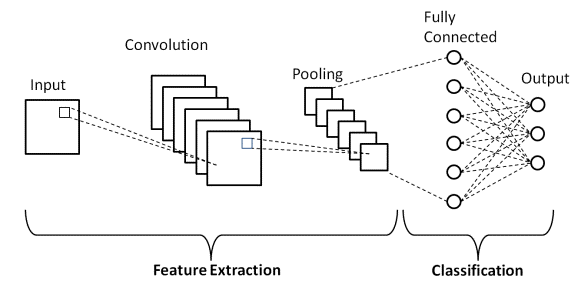
\includegraphics[width=\linewidth, height=10cm,keepaspectratio]{figures/CNN.png}
	\caption{CNN Architecture}
\end{figure}	

\emph{Layers} are the building components of deep neural networks such as CNN and others. A \emph{layer} is a broad phrase that refers to a group of "nodes" that function together at a given level within a neural network. \emph{Layers} are classified into three types: \emph{input layer},\emph{ hidden layers}, and \emph{output layers}.

The \emph{input layer} contains raw data (each variable as a "node") \\
In neural networks, black magic happens in the \emph{hidden layer}(s). By minimizing an error/cost function, each layer attempts to learn different elements of the data. The context of "image recognition", such as a face, is the most intuitive way to understand these levels. The first layer may learn edge detection, the second eye, the third nose, and so on. This isn't exactly what's going on, but the idea is to split the problem down into components that different levels of abstraction can piece together, much to how our own brains work (hence the name neural networks).

The \emph{output layer} is the simplest, usually consisting of a single output for classification problems. Even though it is a single "node", it is nevertheless regarded as a layer in a neural network because it might contain numerous nodes. We use six types of layers given by the TensorFlow framework in this thesis: \textbf{Embedding} layer, \textbf{Conv1D} layer, \textbf{MaxPooling1D} layer, \textbf{Dropout} layer, \textbf{Flatten} layer, and \textbf{Dense} layer.
\newpage
\subsection{Gradient descent}
\label{subsec:gradient_descent}
\emph{Gradient descent} is an optimization algorithm that is used to minimize a function by iteratively traveling in the direction of the steepest descent as defined by the gradient's negative. Gradient descent\index{Gradient descent} is used in machine learning\index{Machine learning (ML)} to update the parameters of our model, especially weights in neural networks.
\begin{figure}[!h]
	\centering
	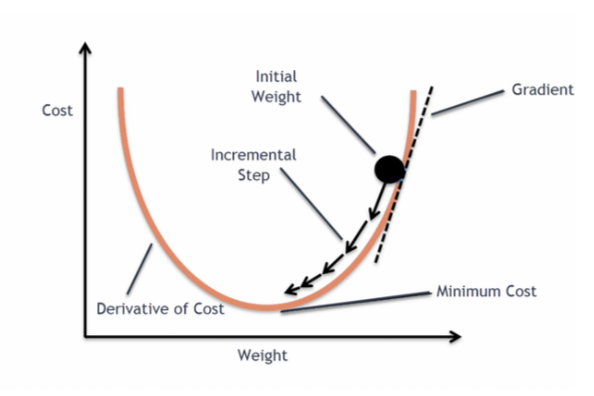
\includegraphics[width=\linewidth, height=10cm,keepaspectratio]{figures/gradient descent.png}
   \caption{Gradient descent demonstration}
\end{figure}
\subsection{Learning Rate}
\label{subsec:learning_rate}
The learning rate\index{Learning rate} is the size of each step in each gradient descent cycle. We can cover more territory per step with a high learning rate, but we risk overshooting the lowest spot because the slope of the hill is continually changing. We may reliably go in the direction of the negative gradient with a very low learning rate because we are recalculating it so frequently. A low learning rate is more exact, but calculating the gradient takes time, so we will take a long time to reach the bottom. An example of the learning rate is in Figure 2.5.
\newpage
\begin{figure}[!h]
	\centering
	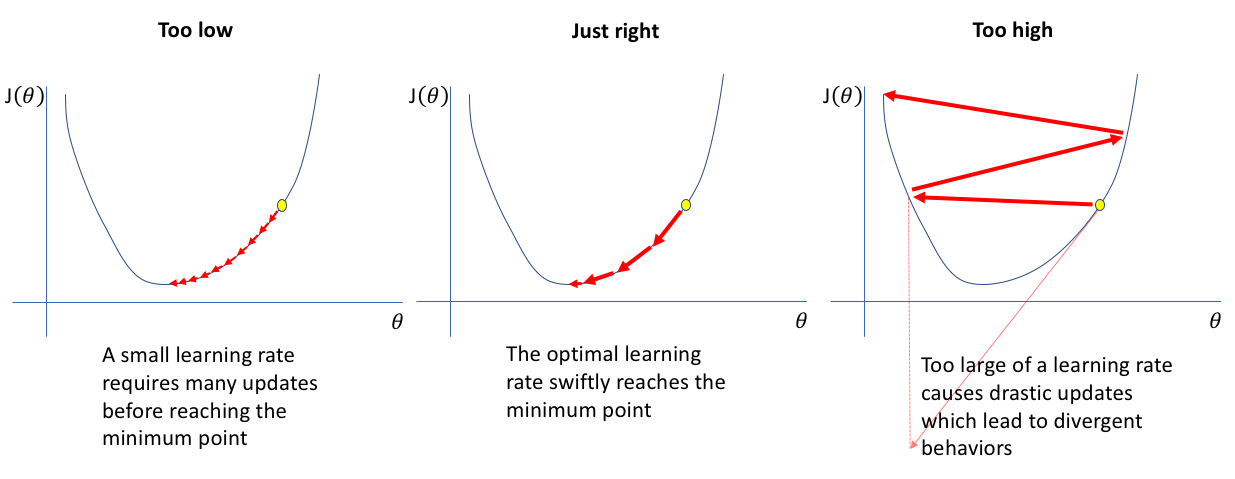
\includegraphics[width=\linewidth, height=10cm,keepaspectratio]{figures/learning rate.png}
   \caption{Learning rate}
\end{figure}

\subsection{Loss Function}
\label{subsec:loss_function}
A Loss Function\index{Loss function} (or cost function) indicates how well the model predicts a given set of parameters. Index of the cost function The loss function has its curve and gradients. The slope of this curve indicates how we should adjust our parameters to improve the model's accuracy\index{Accuracy}. If the cost ever rises, we must reduce the value of the learning rate\index{Learning rate}; if the cost falls slowly, we must increase the value of the learning rate. Figure 2.6 shows examples of loss function behavior based on the learning rate.
\begin{figure}[!h]
	\centering
	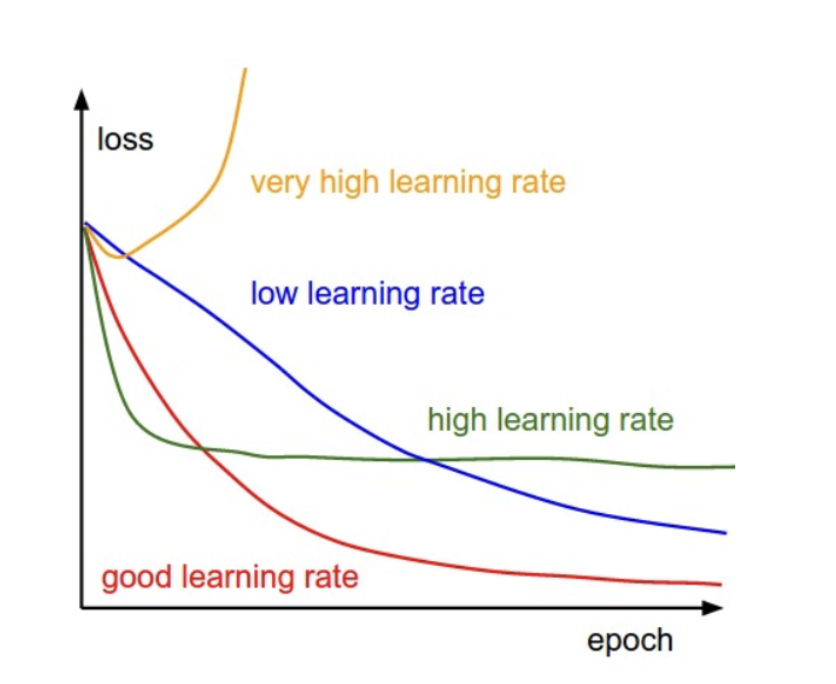
\includegraphics[width=\linewidth, height=10cm,keepaspectratio]{figures/loss function DL.png}
   \caption{Loss function behaviour with different learning rate}
\end{figure}

\subsection{Gradient descent optimizer}
\label{gradient_optimizer}
A method that computes adaptive learning rates\index{Learning rate} for each parameter is Adaptive Moment Estimation (Adam). Adam\index{Adam (algorithm)}, like Adadelta and RMSprop, preserves an exponentially decaying average of past squared gradients $v_t$ in addition to an exponentially decaying average of past gradients $m_t$. Whereas momentum can be thought of as a ball rolling down a hill, Adam behaves more like a heavy ball with friction, preferring flat minima on the error surface. The decaying averages of past and past squared gradients, $m_t$ and $v_t$, are computed as follows:
\begin{align}
    m_t \: = \: \beta_1 m_{t-1} \: + \: (1-\beta_1)g_{t}\\
    v_t \: = \: \beta_2 v_{t-1} \: + \: (1-\beta_2)g^2_t
\end{align}


$m_t$ and $v_t$ are estimates of the first moment (the mean) and the second moment (the uncentered variance) of the gradients respectively, hence the name of the method. As $m_t$ and $v_t$ are initialized as vectors of 0's, the authors of Adam observe that they are biased towards zero, especially during the initial time steps, especially when the decay rates are small.
\begin{align}
    \hat{m}_t \: = \: \frac{m_t}{1\:-\:\beta^t_1} \\
 \hat{v}_t \: = \: \frac{v_t}{1\: - \: \beta^t_2}
\end{align}



They then use these to update the parameters:
\begin{align}
\theta_{t+1} \: = \: \theta_t \: - \: \frac{\eta}{\sqrt{\hat{v}_t} \: +\: \epsilon} \hat{m}_t 
\end{align}
